\renewcommand{\thesubsubsection}{\alph{subsubsection})}
\setcounter{section}{4}
\setcounter{subsection}{0}
\renewcommand{\thesubsubsection}{\alph{subsubsection})}

\subsection{Stride access (30 pts)}
\subsubsection{Direct-mapped cache, $s=1$ $n=8$}
The cache is direct-mapped, has blocks of size 32 bytes and a total capacity of 1 KiB. This means that there are $\frac{2^{10}}{32} = 32$ cache blocks. Each cache block/line contains 32 bytes (4 doubles).\\

The access pattern of matrix $O$ is the following: Each element is accessed sequentially from row $0$ to row $n-3=5$. Therefore in total there are 12 compulsory cache misses, two for each row of $O$.

Regarding the access pattern of $A$ instead, at each iteration, the corresponding elements at row $i-1$ and $i+1$ are accessed. Similar to before we only have 16 compulsory cache misses, two for each row of $A$.

We have a total of 192 memory accesses. 28 of which are compulsory cache misses, after which all the rows of $A$ and $O$ are in the cache. Therefore the cache miss rate is $\frac{28}{192}  = 14.583333\%$.\vspace*{-0.4cm}
\subsubsection{Direct-mapped cache, $s=2$ $n=16$}
The cache structure is analagous as before. The main difference is that since matrix $A$ and $O$ are $16\times16$, the cache can only store exactly half of one of them at a time. Therefore, elements from $A$ and $O$ with the same coordinates map to the same cache location.\\
By increasing the stride to 2, not every element of $A$ is accessed. In fact, the columns are covered in an alternating pattern, resulting in only half of the elements being accessed. Matrix $O$ is still accessed in a sequential manner.

In the first 4 iterations, the cache gets repeatedly evicted because the first 4 elements of $O$ share the same cache block as the first elements of $A$. After the initial 4 iterations, this light form of thrashing stops, resulting only in compulsory cache misses.

We have 112 iterations and a total of 448 memory accesses, 107 of which are cache misses, therefore the cache miss rate is $\frac{107}{448} = 23.883929\%$.\vspace*{-0.4cm}

\subsubsection{2-way associatice cache, $s=2$ $n=16$}
% TODO: Idk wtf Im writing here
Since the cache is 2-way associative, it has 16 sets with 2 cache lines each. Each row of $A$ and $O$ is 16 doubles, meaning that two cache blocks are needed to store one full row.

We have 112 iterations and a total of 448 memory accesses, 92 of which are cache misses, therefore the cache miss rate is $\frac{92}{448} = 20.535714\%$.\vspace*{-0.4cm}


% total accesses  = 8*8 + 8*6 = 112
\subsection{Cache mechanics (20 pts)}
\subsubsection{Access patterns and state of direct-mapped cache}
\begin{enumerate}[label=\roman*. ]
\item Cache at line 18\\
\begin{table}[h!]
\begin{tabular}[t]{l}
    i = 0\\
    x: \textbf{MMM}\\
    y: \textbf{MMM}\\
\end{tabular}
\begin{tabular}[t]{|c|c|}
    Set & Block 0 \\ \hline
    0 & $y_2.a$\quad$y_2.b$ \\ \hline
    1 & - \\ \hline
    2 & - \\ \hline
    3 & - \\ \hline
    4 & $x_2.a$\quad$x_2.b$ \\ \hline
    5 & - \\ \hline
    6 & - \\ \hline
    7 & - \\ \hline
    \end{tabular}
\end{table}\\
\begin{table}[h!]
    \begin{tabular}[t]{l}
        i = 1\\
        x: \textbf{HHH}\\
        y: \textbf{MHH}\\
    \end{tabular}
    \begin{tabular}[t]{|c|c|}
    Set & Block 0 \\ \hline
    0 & $y_2.a$\quad$y_2.b$ \\ \hline
    1 & - \\ \hline
    2 & $y_3.a$\quad$y_3.b$ \\ \hline
    3 & - \\ \hline
    4 & $x_2.a$\quad$x_2.b$ \\ \hline
    5 & - \\ \hline
    6 & - \\ \hline
    7 & - \\ \hline
    \end{tabular}
\end{table}\\
\item Cache at line 30\\
\begin{table}[h!]
    \begin{tabular}[t]{l}
        i = 0\\
        x: \textbf{MMM}\\
        y: \textbf{MMM}\\
    \end{tabular}
    \begin{tabular}[t]{|c|c|}
    Set & Block 0 \\ \hline
    0 & $y_2.a$\quad$y_2.b$ \\ \hline
    1 & $y_6.c$\quad$y_6.d$ \\ \hline
    2 & $y_3.a$\quad$y_3.b$ \\ \hline
    3 & $x_5.c$\quad$x_5.d$ \\ \hline
    4 & $x_2.a$\quad$x_2.b$ \\ \hline
    5 & $y_0.c$\quad$y_0.d$ \\ \hline
    6 & - \\ \hline
    7 & - \\ \hline
    \end{tabular}
\end{table}\\
\begin{table}[h!]
    \begin{tabular}[t]{l}
        i = 1\\
        x: \textbf{MMM}\\
        y: \textbf{MHM}\\
    \end{tabular}
    \begin{tabular}[t]{|c|c|}
    Set & Block 0 \\ \hline
    0 & $y_2.a$\quad$y_2.b$ \\ \hline
    1 & $y_6.c$\quad$y_6.d$ \\ \hline
    2 & $y_3.a$\quad$y_3.b$ \\ \hline
    3 & $y_3.c$\quad$y_3.d$ \\ \hline
    4 & $x_2.a$\quad$x_2.b$ \\ \hline
    5 & $x_2.c$\quad$x_2.d$ \\ \hline
    6 & - \\ \hline
    7 & - \\ \hline
    \end{tabular}
    \end{table}\\
\end{enumerate}
\clearpage
\subsubsection{Access patterns and state of 2-way associative cache}
\begin{enumerate}[label=\roman*. ]
\item Cache at line 18\\
\begin{table}[h!]
    \begin{tabular}[t]{l}
        i = 0\\
        x: \textbf{MMM}\\
        y: \textbf{MMM}\\
    \end{tabular}
    \begin{tabular}[t]{|c|c|c|}
    Set & Block 0 & Block 1 \\ \hline
    0 & $x_2.a$\quad$x_2.b$ & $y_2.a$\quad$y_2.b$ \\ \hline
    1 & - & - \\ \hline
    2 & - & - \\ \hline
    3 & - & - \\ \hline
    \end{tabular}
\end{table}\\
\begin{table}[h!]
    \begin{tabular}[t]{l}
        i = 1\\
        x: \textbf{HHH}\\
        y: \textbf{MHH}\\
    \end{tabular}
    \begin{tabular}[t]{|c|c|c|}
    Set & Block 0 & Block 1 \\ \hline
    0 & $x_2.a$\quad$x_2.b$ & $y_2.a$\quad$y_2.b$ \\ \hline
    1 & - & - \\ \hline
    2 & $y_3.a$\quad$y_3.b$ & - \\ \hline
    3 & - & - \\ \hline
    \end{tabular}
\end{table}
\item Cache at line 30\\
\begin{table}[h!]
    \begin{tabular}[t]{l}
        i = 0\\
        x: \textbf{MMM}\\
        y: \textbf{MMM}\\
    \end{tabular}
    \begin{tabular}[t]{|c|c|c|}
    Set & Block 0 & Block 1 \\ \hline
    0 & $x_2.a$\quad$x_2.b$ & $y_2.a$\quad$y_2.b$ \\ \hline
    1 & $y_6.c$\quad$y_6.d$ & $y_0.c$\quad$y_0.d$ \\ \hline
    2 & $y_3.a$\quad$y_3.b$ & - \\ \hline
    3 & $x_5.c$\quad$x_5.d$ & - \\ \hline
    \end{tabular}
\end{table}\\
\begin{table}[h!]
    \begin{tabular}[t]{l}
        i = 1\\
        x: \textbf{MMH}\\
        y: \textbf{MMH}\\
    \end{tabular}
    \begin{tabular}[t]{|c|c|c|}
    Set & Block 0 & Block 1 \\ \hline
    0 & $x_2.a$\quad$x_2.b$ & $y_2.a$\quad$y_2.b$ \\ \hline
    1 & $x_2.c$\quad$x_2.d$ & $y_6.c$\quad$y_6.d$ \\ \hline
    2 & $y_3.a$\quad$y_3.b$ & - \\ \hline
    3 & $x_5.c$\quad$x_5.d$ & $y_3.c$\quad$y_3.d$ \\ \hline
    \end{tabular}
    \end{table}
\end{enumerate}
\subsection{Rooflines (40 pts)}
\subsubsection{Roofline plot}
\begin{figure}[h!]
    \centering
    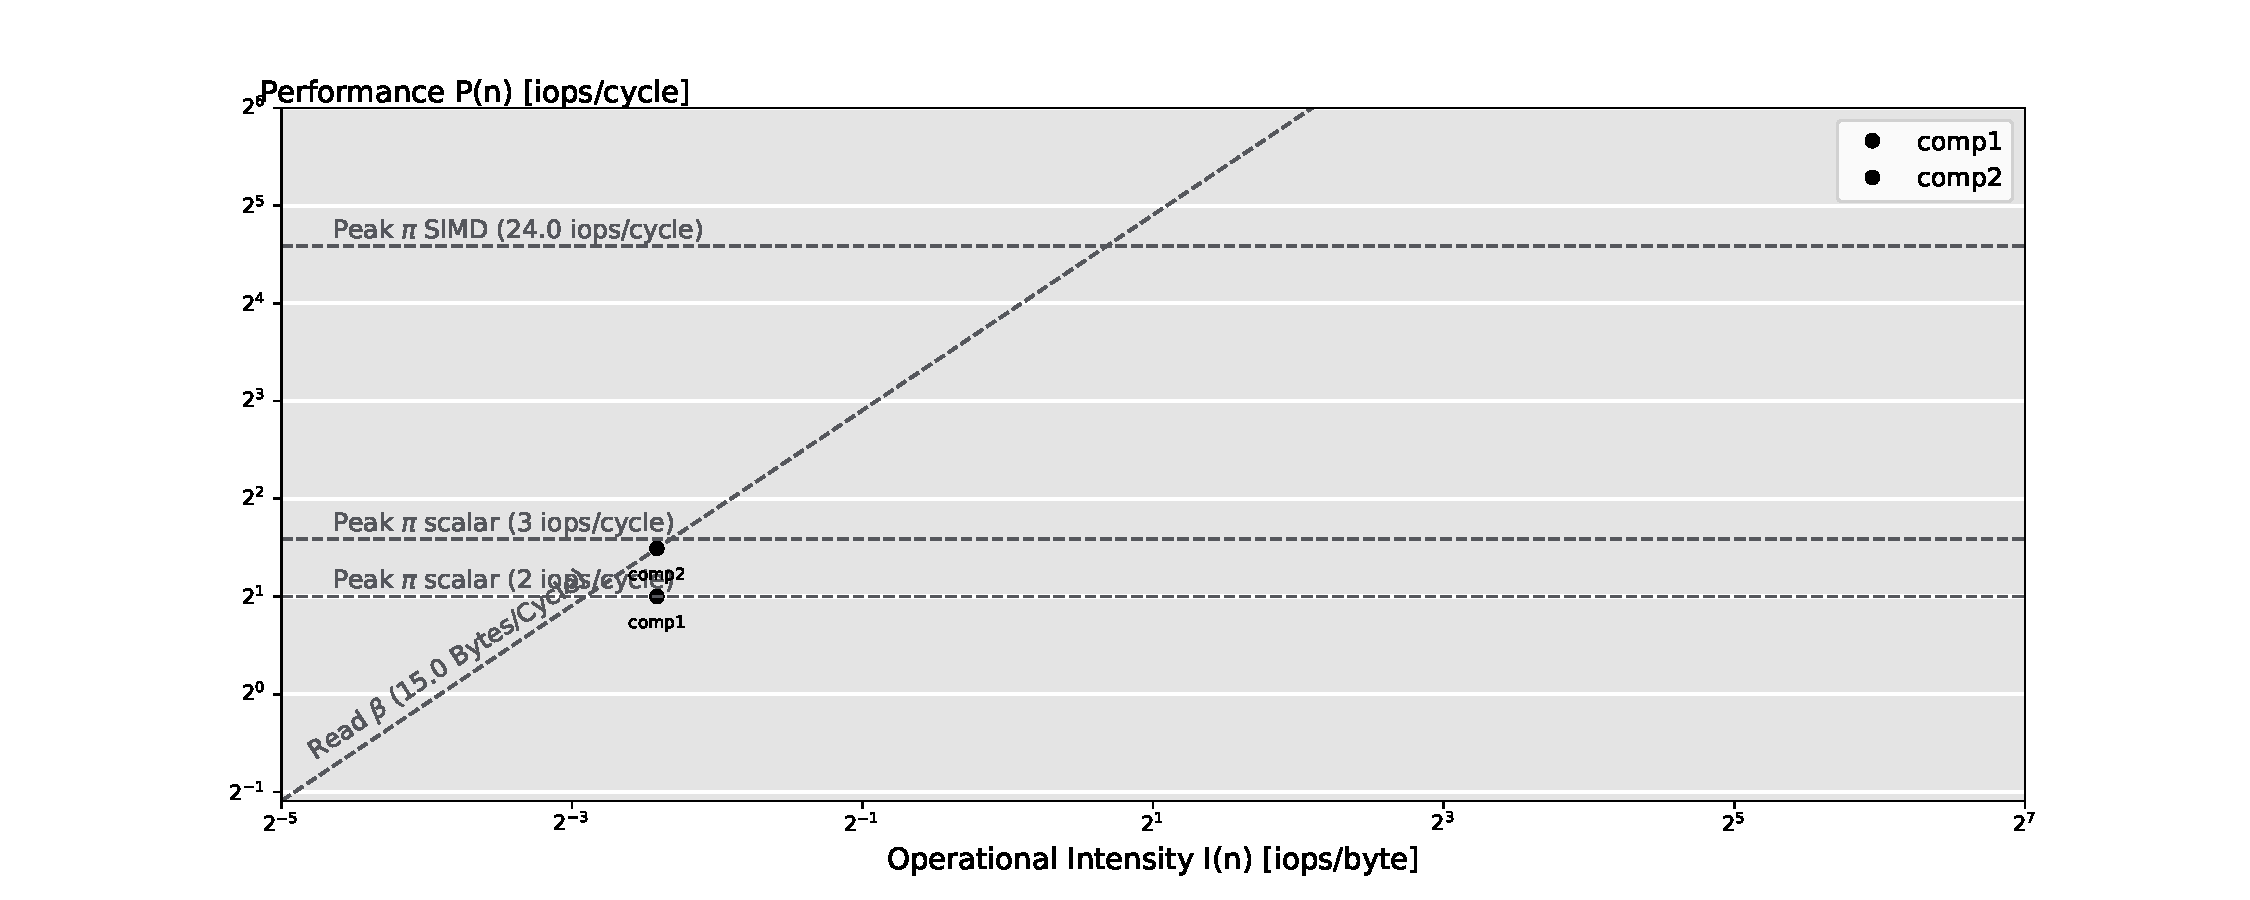
\includegraphics[width=\linewidth]{../out/ex3a.pdf}
\end{figure}
\subsubsection{Scalar performance bounds}

\subsubsection{SIMD performance bounds}


\subsection{Cache miss analysis (25 pts)}

